\chapter{The numerical model EULAG}
\label{sec:EULAG}
The nonlinear numerical simulations are conducted with the EUlerian/semi- LAGrangian fluid solver (EULAG). EULAG was written by Piotr Smolarkiewicz, but many others contributed to the code. The research code is comprised in one file combining two programming languages, shell script and FORTRAN (mostly FORTRAN 77), to create a very fast executable program. A comprehensive description of the algorithm is given in \textcite[]{smolarkiewicz_forward--time_1997} and \textcite[]{smolarkiewicz_mpdata_1998}. \\
EULAG has a proven itself as a reliable tool for simulating thermo-fluid flows across the wide range from turbulent to global scales (\cite{prusa_all-scale_2003}) and in a variety of physical scenarios like e.g. turbulence, GW dynamics, flows past complex/moving boundaries, micrometeorology or cloud microphysics (\cite{prusa_eulag_2008}). A comparison between different well-established numerical models (including EULAG) and their capability to model flow over steep terrain, which is relevant for the investigations within this thesis, appears in \textcite{doyle_intercomparison_2011}.

The underlying setup of EULAG for this work is described in the first section of this chapter \ref{sec:eulag-setup}. It follows a more detailed description of relevant atmospheric background conditions in section \ref{sec:ambient-profiles} and the implementation of a transient lower boundary for the idealized simulations is explained in section \ref{sec:trans-boundary}. Section \ref{sec:linear-MWs} completes this chapter with a comparison of non-linear EULAG simulations to analytic results from linear theory for different MW scenarios. It serves as an additional validation of EULAG before using it for the investigation of NOGWs above propagating tropopause folds.

%%%%%%%%%%%% General setup %%%%%%%%%%%%%%%%
\section{General setup}
\label{sec:eulag-setup}
The model is set up solving the soundproof anelastic set of equations (\cite{lipps_scale_1982}) consisting of the three components of the momentum equation (\ref{equ:momEqu}), the thermodynamic equation (\ref{equ:potTemp}) for the potential temperature perturbation $\Theta'=\Theta-\Theta_e$ and the mass continuity equation (\ref{equ:continuityEqu}):
%
\begin{equation}
\begin{aligned}
    \frac{d \Vec{v}}{dt} = -G \Vec{\nabla} \biggl(\frac{p'}{\rho_0}\biggr) +  \Vec{g} \frac{\Theta'}{\Theta_0} - 2 \Vec{\Omega} \times \bigl(\Vec{v}-\Vec{v_e}\bigr) - \Tilde{\alpha} \bigl(\Vec{v}-\Vec{v_e}\bigr) \equiv R^{v},
    \label{equ:momEqu}
\end{aligned}
\end{equation}
\begin{equation}
    \frac{d \Theta'}{dt} = -\Vec{v} \cdot \Vec{\nabla} \Theta_e - \Tilde{\beta} \bigl(\Theta-\Theta_e\bigr) \equiv R^{\Theta},
    \label{equ:potTemp}
\end{equation}
\begin{equation}
    \Vec{\nabla} \cdot \bigl(\rho_0 \Vec{v}\bigr) = 0.
    \label{equ:continuityEqu}
\end{equation}
%
Here, $\frac{d}{dt}$, $\Vec{\nabla}$ and $\Vec{\nabla} \cdot$ represent the total derivative, the gradient and the divergence respectively. $p'$ is the pressure perturbation with respect to the environmental state, g the gravitational acceleration and $\Vec{\Omega}$ the angular velocity of the Earth. The matrix G represents geometric terms, which result from the general, time-dependent coordinate transformation and the symbol $R^{\Psi}$ stands for the right-hand side of the corresponding equations for the variables $\Psi = (u,v,w,\Theta')$. \\
$\rho_0(z)$ and $\Theta_0(z)$ refer to the hydrostatic reference state or basic state of equations (\ref{equ:momEqu}-\ref{equ:continuityEqu}). EULAG provides multiple options to define this reference state of the atmosphere including one that is well suited for modelling deep atmospheres following \textcite{bacmeister_breakdown_1989}. A more general environmental state, which reflects the initial and boundary conditions, enters the equations via the variables with subscript e. These ambient states like $u_e$, $\rho_e$ or $\Theta_e$ can relate to the reference state, but they can also be time-dependent to replicate transient flow conditions. In that sense, $\alpha(\Vec{v}-\Vec{v_e})$ and $\beta(\theta-\theta_e)$ represent relaxation terms, which enable the radiation of wave energy across the model boundaries and force the solutions at the boundaries to the prescribed environmental profiles. Both, reference and environmental profiles are described in detail in the following section \ref{sec:ambient-profiles}. \\
A particularly useful feature of EULAG for our simulations is the possibility for transient boundaries (\cite[]{prusa_propagation_1996} and \cite{wedi_extending_2003}). We will use this option to mimic a propagating tropopause fold at the lower boundary and to avoid unphysical, transient processes during the initialization of the simulation. More details follow in section \ref{sec:trans-boundary}. Furthermore, EULAG is noteworthy for its robust elliptic solver (\cite{smolarkiewicz_forward--time_1993}) and generalized coordinate formulation enabling grid adaptivity technology (\cite{prusa_eulag_2008}, \cite{kuhnlein_modelling_2012}).

\subsection*{Numerics}
As the name suggests, EULAG is capable of solving the equations of motion (\ref{equ:momEqu}-\ref{equ:continuityEqu}) in an Eulerian (flux form) or in a semi-Lagrangian (advective form) mode (\cite{smolarkiewicz_forward--time_1997}). For the numerical approximation it utilizes a non-oscillatory forward-in-time (NFT) approach compactly formulated as
\begin{equation}
\begin{aligned}
    \Psi^{n+1} = LE(\Tilde{\Psi}, V^{n+1}, G^n, G^{n+1}) \\
    + \frac{1}{2} \Delta t R^{\Psi} |^{n+1}
    \label{equ:NFTscheme}
\end{aligned}
\end{equation}
with $LE$ representing the corresponding semi-Lagrangian/Eulerian transport operator. The NFT scheme belongs to the class of second-order-accurate two-time-level algorithms that are build on nonlinear advection techniques (\cite{prusa_eulag_2008}). These schemes have the property to suppress and control numerical oscillations that are often found in higher order linear schemes. As a result, transporting the auxiliary field $\Tilde{\Psi} = \Psi^n + \frac{1}{2} \Delta t R^{\Psi}|^n$ instead of the specific variable $\Psi$, results from a thorough truncation error analysis and ensures second order accuracy. (\cite{smolarkiewicz_forward--time_1997}). Within the scope of this Master's thesis all simulations utilize the Eulerian option by applying the multidimensional positive definite advection transport algorithm MPDATA (\cite{smolarkiewicz_mpdata_1998} and \cite{smolarkiewicz_multidimensional_2006}).

%%%%% NOTES %%%%%

% Prusa 2008 also has good description of perturbation form and points out importance of correct environmental/initial state!! 

% \cite{smolarkiewicz_multidimensional_2006}

% \begin{equation}
%    \frac{\partial G \rho \Psi}{\partial t} + \nabla \cdot G \rho \Vec{v} = G \rho R
%    \label{equ:statMeshAdapt}
% \end{equation}


% he elliptic pressure equation is solved via a preconditioned non-symmetric Krylov sub- space solver (Smolarkiewicz and Margolin; 1994; 1997, Skamarock et al., 1997).

% imlicit /explicit elliptic pressure solver / krylov sub space solver

% There, governing equations are formulated in general- ized time-dependent curvi-linear coordinates to enable mesh adaptivity (Prusa and Smolarkiewicz 2003; Wedi and Smolarkiewicz 2004; Kühnlein et al. 2012; Smolarkiewicz and Charbonneau 2013) and continuous mappings of the Earth’s topography by using terrain-following coordinates (Gal-Chen and Somerville 1975; Clark 1977)


% anelastic -> elastic energy is not allowed -> sound waves are filtered since they are based on pressure difference rather then temperature

%%%%%%%%%%%% Ambient profiles %%%%%%%%%%%%%%%%
\section{Ambient profiles of idealized simulations}
\subsection*{The hydrostatic reference state: Bacmeister-Schoeberl Model}
\begin{figure*}[tbp]
    \centering
    \includegraphics[width=0.45\textwidth]{figures_model/bac-schoeber-ambient-profiles.png}
    \caption{Vertical profiles of ambient pressure $p_0$ (orange), density $\rho_0$ (blue), absolute temperature $T_0$ (red) and potential temperature $\Theta_0$ (purple) scaled by corresponding surface values for the isothermal atmosphere described by \textcite[]{bacmeister_breakdown_1989}.}
    \label{fig:ambient_profs}
\end{figure*}
\label{sec:ambient-profiles}
The anelastic equations (\ref{equ:momEqu}-\ref{equ:continuityEqu}) rely on hydrostatically balanced reference profiles of the dependent variables ($\rho$, $p$ and $\Theta$) that vary with height, but not horizontally or in time. For the presented idealized simulations these reference profiles (subscript 0 in the previous section) define an isothermal atmosphere with constant stability following \textcite{bacmeister_breakdown_1989}. In the anelastic framework it is only necessary to define the vertical profile of potential temperature and a reference pressure $p_{00}$. All other variables follow from the definition of $\Theta$
\begin{equation}
    \Theta(z) = T(z) \biggl(\frac{p_{0}}{p}\biggr)^{\kappa},
    \label{equ:poissonEqu}
\end{equation}
the ideal gas law
\begin{equation}
    \rho(z) = \frac{p(z)}{R T(z)}
    \label{equ:idealGas}
\end{equation}
and the assumption of hydrostatic balance $\frac{dp}{dz}=-\rho g$ that results in
% general equation in 
\begin{equation}
    \frac{1}{\rho} \frac{d \rho}{dz} + \frac{1}{\Theta} \frac{d \Theta}{dz} = \frac{\kappa-1}{H_{\rho}} \biggl(\frac{\rho}{\rho_0} \biggr)^{\frac{\kappa}{\kappa-1}} \biggl(\frac{\Theta}{\Theta_0} \biggr)^{\frac{1}{\kappa-1}}
    \label{equ:hydro-balance}
\end{equation}
and can be solved for a density profile $\rho(z)$ after defining the potential temperature profile $\Theta(z)$. For the isothermal atmosphere of \textcite[]{bacmeister_breakdown_1989} it provides $H_{\rho} = \kappa H_{\Theta}$ and the reference profiles (Figure \ref{fig:ambient_profs})
\begin{equation}
    \begin{aligned}
        \Theta_0(z) &= T_{00} e^{\frac{z}{H_{\Theta}}} \quad \textrm{with} \quad H_{\Theta} = \frac{g}{N^2} = \frac{c_p T_{00}}{g}, \\
        \rho_0(z) &= \rho_{00} e^{-\frac{z}{H_{\rho}}} \quad \textrm{with} \quad H_{\rho} = \frac{R T_{00}}{g} \quad \textrm{and}  \\
        p_0(z) &= p_{00} e^{-\frac{z}{H_{\rho}}}
        \label{equ:ambient-profiles}
    \end{aligned}
\end{equation}
with the Brunt-Vaisala frequency $N=\bigl(\frac{g}{\Theta}\frac{\partial \bar{\Theta}}{\partial z}\bigr)^{\frac{1}{2}}$, the specific gas constant $R$ and the specific heat capacity at constant pressure $c_p$. These exponential profiles avoid physical restrictions towards higher altitudes (compare Figure \ref{fig:ambient_profs}) and are thus well suited for the investigation of deep gravity wave propagation. \\
All relevant parameters for these ambient profiles used for our simulations are summarized in Table \ref{tab:ambientProfiles}. Values for the troposphere are used for EULAG simulations of linear MW scenarios in section \ref{sec:linear-MWs}, values for the stratosphere are used for all simulations of a propagating tropopause fold in chapters \ref{sec:resultsQ3D} and \ref{sec:results3D}. The fact that there are two columns for the troposphere emphasizes a quite unrealistic relation of the isothermal temperature $T_{00}$ and $\kappa$ for a tropospheric Brunt-Väisälä frequency of $N=\SI{0.01}{\per\second}$. Based on the definition of $H_{\Theta}$ and $H_{\rho}$ choosing $\kappa=\frac{2}{7}$ to represent diatomic gases results in a very high temperature $T_{00} = \SI{957}{K}$. For a more realistic temperature $T_{00} = \SI{274}{K}$ $\kappa$ has to be reduced to $\kappa=\frac{2}{24.4}$. When using the soundproof anelastic equations similar to \textcite[]{lipps_scale_1982} the choice of $\kappa$ and $T_{00}$ is not affecting energy and momentum fluxes, so both descriptions of the troposhere in Table \ref{tab:ambientProfiles} lead to the same result in section \ref{sec:linear-MWs}. This has been tested, too. For simulations of the stratosphere with $N=\SI{0.02}{\per\second}$ a $\kappa$ for diatomic gases leads to a reasonable temperature of $T_{00} = \SI{239}{K}$.
\begin{table*}[ht]
\centering
\caption{Summary of parameters related to the vertical profiles of the ambient reference state following \textcite[]{bacmeister_breakdown_1989}. Values for the troposphere are used for the model validation in section \ref{sec:linear-MWs}. Values for the stratosphere are used for simulations of a propagating tropopause fold in chapters \ref{sec:resultsQ3D} and \ref{sec:results3D}. The first troposphere column is for a reasonable temperature $T_{00}$, the second troposphere column is for a diatomic gas. Grey rows refer to parameters that need to be defined.}
\begin{tabular}{@{}ccccc@{}}
\toprule
 & Unit & Troposphere & Troposphere ($\kappa=\frac{2}{7}$) & Stratosphere \\ \midrule[1pt]

 \rowcolor{LightCyan} $R$ & J kg$^{-1}$ K$^{-1}$ &   \cellcolor{LightCyan} 287.04 &   \cellcolor{LightCyan} 287.04 &   \cellcolor{LightCyan} 287.04 \\
 \rowcolor{LightCyan} $g$ & m s$^{-2}$ & \cellcolor{LightCyan} 9.80616 & \cellcolor{LightCyan} 9.80616 & \cellcolor{LightCyan} 9.80616 \\
 \rowcolor{LightCyan} $N$ & s$^{-1}$ & \cellcolor{LightCyan} 0.01 & \cellcolor{LightCyan} 0.01 & \cellcolor{LightCyan} 0.02 \\
\rowcolor{LightCyan} $\kappa$ & - & $\frac{2}{24.4}$ & $ \frac{2}{7}$ & $ \frac{2}{7}$ \\
$c_p$ & J kg$^{-1}$ K$^{-1}$ & $\frac{24.4}{2} R$ & $\frac{7}{2} R$ & $\frac{7}{2} R$ \\
$H_{\Theta}$ & m & 98061.6 & 98061.6 & 24515.4  \\
$H_{\rho}$ & m & 8011.3  & 28017.6  & 7004.4 \\

& & & & \\
\rowcolor{LightCyan} $p_{00}$ & Pa & \cellcolor{LightCyan} $1.01 \times 10^5$ & \cellcolor{LightCyan} $1.01 \times 10^5$ & \cellcolor{LightCyan} $0.235 \times 10^5$ \\
$T_{00}$ & K & 273.69 & 957.17 & 239.39 \\
$\rho_{00}$ & kg m$^{-3}$ & 1.2856 & 0.3676 & 0.3454 \\

\bottomrule
\end{tabular}
\label{tab:ambientProfiles}
\end{table*}

Ambient profiles (subscript $e$ in the anelastic equations (\ref{equ:momEqu}-\ref{equ:continuityEqu})) of the dependent variables ($\rho_e$, $p_e$ and $\Theta_e$) are stationary (not time-dependent) and therefore identical to the vertical profiles of the hydrostatic reference state (subscript 0).

\subsection*{Ambient wind profiles}
All presented simulations are conducted in 3D, but enforce a purely zonal background flow $u_e(z,y)$ with no meridional background wind $v_e=0$. Nevertheless, meridional perturbations $v'$ develop due to the Coriolis force and the 3D nature of inertia-gravity waves. Some simulations including the model validation in section \ref{sec:linear-MWs} have a constant wind $u_e$ without vertical and meridional shear. In the remaining simulations for the sensitivity study in chapter \ref{sec:resultsQ3D} $u_e(z)$ varies with altitude, but it is still constant in meridional direction. In chapter \ref{sec:results3D} $u_e(z,y)$ is a function of $z$ and $y$ to incorporate the meridional structure of the PNJ. At this point, it is important to note that vertical gradients of the zonal background wind $u_e$ are not coupled to meridional gradients of $\Theta_e$ and $\frac{\partial \Theta_e}{\partial y}=0$ for all simulations. Winds are independent of the potential temperature distribution and in the case of $\frac{\partial u_e}{\partial z} \neq 0$ the thermal wind relation is not fullfilled. Considering the thermal wind relation and simulating a baroclinic instability at tropopause level would be the next step as proposed in the outlook.

\begin{figure*}[tbp]
    \centering
    \includegraphics[width=0.67\textwidth]{figures_model/era5-winds-reichert.png}
    \caption{Illustrated are ERA5 monthly mean absolute wind profiles (thick lines, lower axis) and wind directions above Río Grande (thin lines, upper axis; the dashed lines mark westerlies). The wind field was truncated at T21 in order to filter out contributions from model-resolved GWs. Winter months in the southern hemisphere are blue, summer months red. are The figure is taken from \textcite[]{reichert_characterization_2022}.}
    \label{fig:era5-winds-reichert}
\end{figure*} 
% \cite[]{hindley_radar_2022}
The goal for our simulations was an idealized wind profile typical for the southern hemisphere winter stratosphere with features that can be adjusted individually for a conclusive sensitivity study. A good source of information for the construction of $u_e$ was Figure \ref{fig:era5-winds-reichert} from \textcite[]{reichert_characterization_2022} who analysed monthly means of ERA5 winds above Río Grande at the southern tip of South America (\SI{53.79}{\degree S}) for the years 2017 to 2020. Other sources based on ERA5 data were \textcite[]{rapp_southtrac-gw_2021}, \textcite[]{mixa_nonlinear_2021} and \textcite[]{dornbrack_stratospheric_2022} who also showed profiles from radiosondes and the IFS model (ECMWF) for their case study in the appendix. \\
All show a clear vertical pattern for the winter stratosphere between 50-\SI{60}{\degree S} with a local maximum around the tropopause at 8-\SI{10}{\kilo\meter} (tropopause jet) and a much stronger PNJ at approximately 35-\SI{45}{\kilo\meter} above the tropopause. In most cases, a wind minimum exists above the tropopause jet at approximately 15-\SI{20}{\kilo\meter} (e.g. APR or MAY in Figure \ref{fig:era5-winds-reichert}). This minimum can be more or less pronounced and even vanish (e.g. AUG and SEP for the years 2018 and 2020 in Figure \ref{fig:era5-winds-reichert}) resulting in positive vertical shear throughout the whole stratosphere. Wind maxima of the tropopause jet mostly vary between 35-\SI{55}{\meter\per\second}. The PNJ reaches wind speeds from 60-\SI{140}{\meter\per\second}. \\
To consider and vary these different features independently the idealized vertical profile $u_e(z)$ is a superposition of a base wind U$_0$ and two jet streams (Figure \ref{fig:wind_profs}a) that are both based on a Gaussian distribution
\begin{equation}
    u_e(z) = u_{jet,max} e^{-\frac{1}{2} \bigl(\frac{z-z_{jet}}{\sigma_{jet}}\bigr)^2}
    \label{equ:wind-distribution}
    % squared for symmetric distribution
\end{equation}
with a maximum wind speed $u_{jet,max}$ at $z_{jet}$ and a standard deviation $\sigma_{jet}$ to adjust the vertical gradient $\frac{\partial u_e}{\partial z}$ by making the distribution wider or narrower. In Figure \ref{fig:wind_profs}a the tropopause jet TPJ (purple dashed line) is centered at the lower boundary of the simulation with $\sigma_{jet}=\SI{5}{\kilo\meter}$ and the PNJ (yellow dashed line) is centered at $z_{jet}=\SI{40}{\kilo\meter}$ with $\sigma_{jet}=\SI{13}{\kilo\meter}$. Different parameter combinations result in different vertical profiles of $u_e$, which are compared in section \ref{sec:q3D-wind} and Figure \ref{fig:q3D_wind}.

\begin{figure*}[tbp]
    \centering
    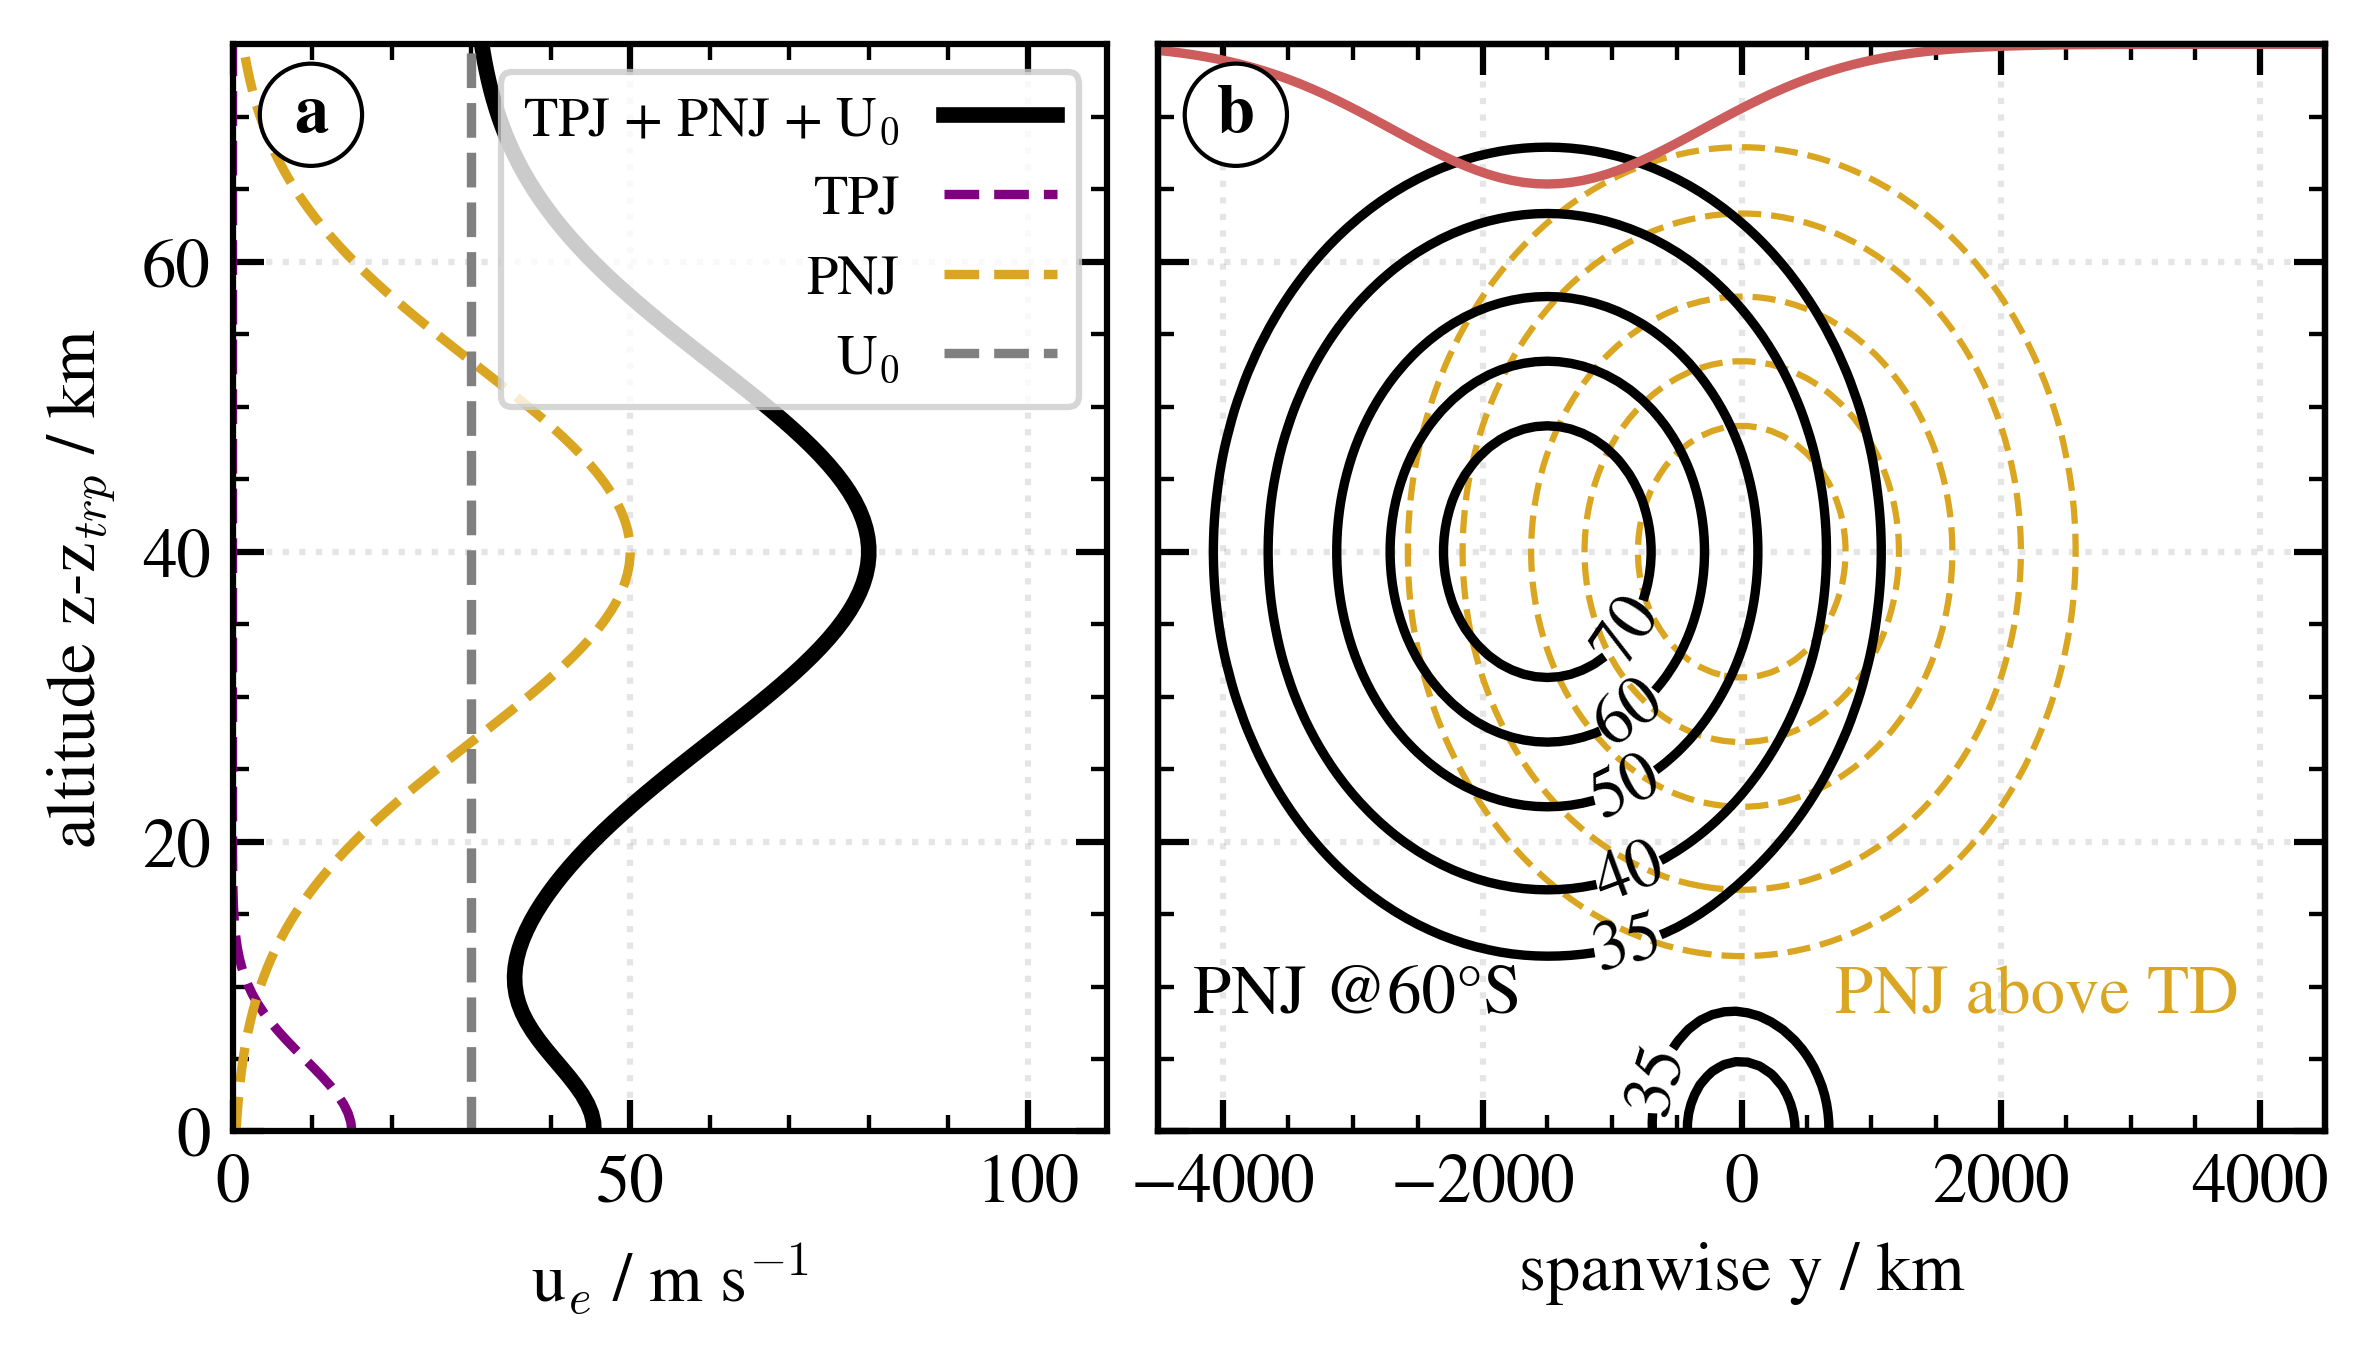
\includegraphics[width=0.75\textwidth]{figures_model/eulag-wind-profiles.png}
    \caption{Vertical profiles of the background wind for EULAG simulations with no meridional shear (a) and with meridional shear (b). The black line in (a) is a superposition of the tropopause jet TPJ (purple), the polar night jet PNJ (yellow) and a base wind U$_0$. Both jet distributions are based on equation (\ref{equ:wind-distribution}). The 2D wind profiles in (b) are obtained by combining the vertical profiles from (a) with a similar distribution in meridional direction (red curve in (b) for the PNJ at 60°S).}
    \label{fig:wind_profs}
\end{figure*} 
%
The meridional position of the PNJ varies during a winter season, but time averages show that it is mostly centered around a latitude of \SI{60}{\degree S} and south of the main stormtrack at tropopause level. To investigate the influence of the PNJ's merdional shear in chapter \ref{sec:results3D}, vertical profiles of $u_e(z)$ are multiplied with a meridional distribution (red line in Figure \ref{fig:wind_profs}b) to obtain variations of $u_e(z,y)$ visualized in Figure \ref{fig:wind_profs}b. The meridional distribution is set up in the same manner as equation \ref{equ:wind-distribution} with a $y_{jet}=\SI{1500}{\kilo\meter}$ and a standard deviation $\sigma_{jet}=\SI{1200}{\kilo\meter}$.

In EULAG idealized wind profiles are implemented within a new subroutine \code{tinit\_idealwind}\footnote[1]{The grey background refers to the name and implementation in the EULAG code.}. 

%%%%%%%%%%%% Transient boundary %%%%%%%%%%%%%%%%
\section{Transient lower boundary of idealized simulations}
\label{sec:trans-boundary}
When solving the anelastic equations (\ref{equ:momEqu}-\ref{equ:continuityEqu}) EULAG allows a time-dependent lower and upper boundary (\cite[]{prusa_propagation_1996} and \cite[]{wedi_extending_2003}). We utilize this feature to bound the numerical simulations at the tropopause and mimic a propagating tropopause fold at the lower boundary. This approach is not new and has already been used by \textcite[]{pfister_gravity_1993} or \textcite[]{prusa_all-scale_2003} to investigate NOGWs above a moving source. \\
The shape of a tropopause fold or, to be more specific, the shape of an isentrope above the tropopause that dips above the fold and rises again (compare with Figure \ref{fig:skerlakFold}) can be approximated by an upside-down isolated mountain.
The Witch of Agnesi
\begin{equation}
    h_{Agnesi}(x) = h_m \frac{L^2}{x^2+L^2}
    \label{equ:agnesi}
\end{equation}
is an established shape to describe isolated mountains in idealized simulations with the crest height $h_m$ and half width $L$. It was already used by \textcite{queney_problem_1948} to derive linear analytic solutions to a range of MW scenarios. Though non-linear simulations with a Witch of Agnesi are compared to Queney's solution in the next section to validate the model, the Witch of Agnesi is not appropriate to simulate a moving obstacle at the lower boundary. The topography following equation \ref{equ:agnesi} is non-zero for the whole domain of a discrete simulation (compare in Figure \ref{fig:topo_trans}). Therefore, the Witch of Agnesi would lead to a constantly changing surface at the domain's horizontal borders and impact the boundary conditions. This makes it a less appropriate shape for a moving topography or transient boundary in simulations. \\
A suitable alternative is a $1+cos(\frac{\pi}{4L}x)$ shape. It drops to 0 for $|\frac{x}{4L}| = 1$, so the sorrounding topography can be set to 0 for $|\frac{x}{4L}| \leq 1$ without sacrificing its continuity and differentiability. This is essential for the implementation of a transient boundary in the model. \textcite[]{prusa_all-scale_2003} already used a variation of the cosine function to mimic a moving tropopause fold in simplified 2D simulations with EULAG, but it exists a variation of the cosine function 
\begin{equation}
    h_{cos}(x) = 
    \begin{cases}
        & \frac{h_m}{16} (1+cos(\frac{\pi}{4L}x))^4, |\frac{x}{4L}| < 1 \\
        & 0, |\frac{x}{4L}| \geq 1 \\
      \end{cases}
    \label{equ:cosMtn}
\end{equation}
with a quite comparable shape to the Witch of Agnesi (equation (\ref{equ:agnesi})). Figure \ref{fig:topo_trans} shows how the shapes compare for a similar half-width and crest height and demonstrates that equation (\ref{equ:cosMtn}) is closest to the Witch of Agnesi. As long as the cosine mountain or depression is not too close to the edges the topography does not interfere with horizontal boundary conditions and all contributions to the surface pressure drag are now confined to a small neighbourhood around the peak. The cosine version of equation (\ref{equ:cosMtn}) has already been used for prescribing idealized topographies in 2D, too (\cite[]{epifanio_three-dimensional_2001} and \cite[]{metz_are_2021}). \textcite{metz_are_2021} state that the linear pressure drag across the cosine mountain of equation (\ref{equ:cosMtn}) is a factor of 1.3 higher compared to a corresponding Witch of Agnesi for a constant $N$ and $U$ environment.
\begin{figure*}[t]
    \centering
    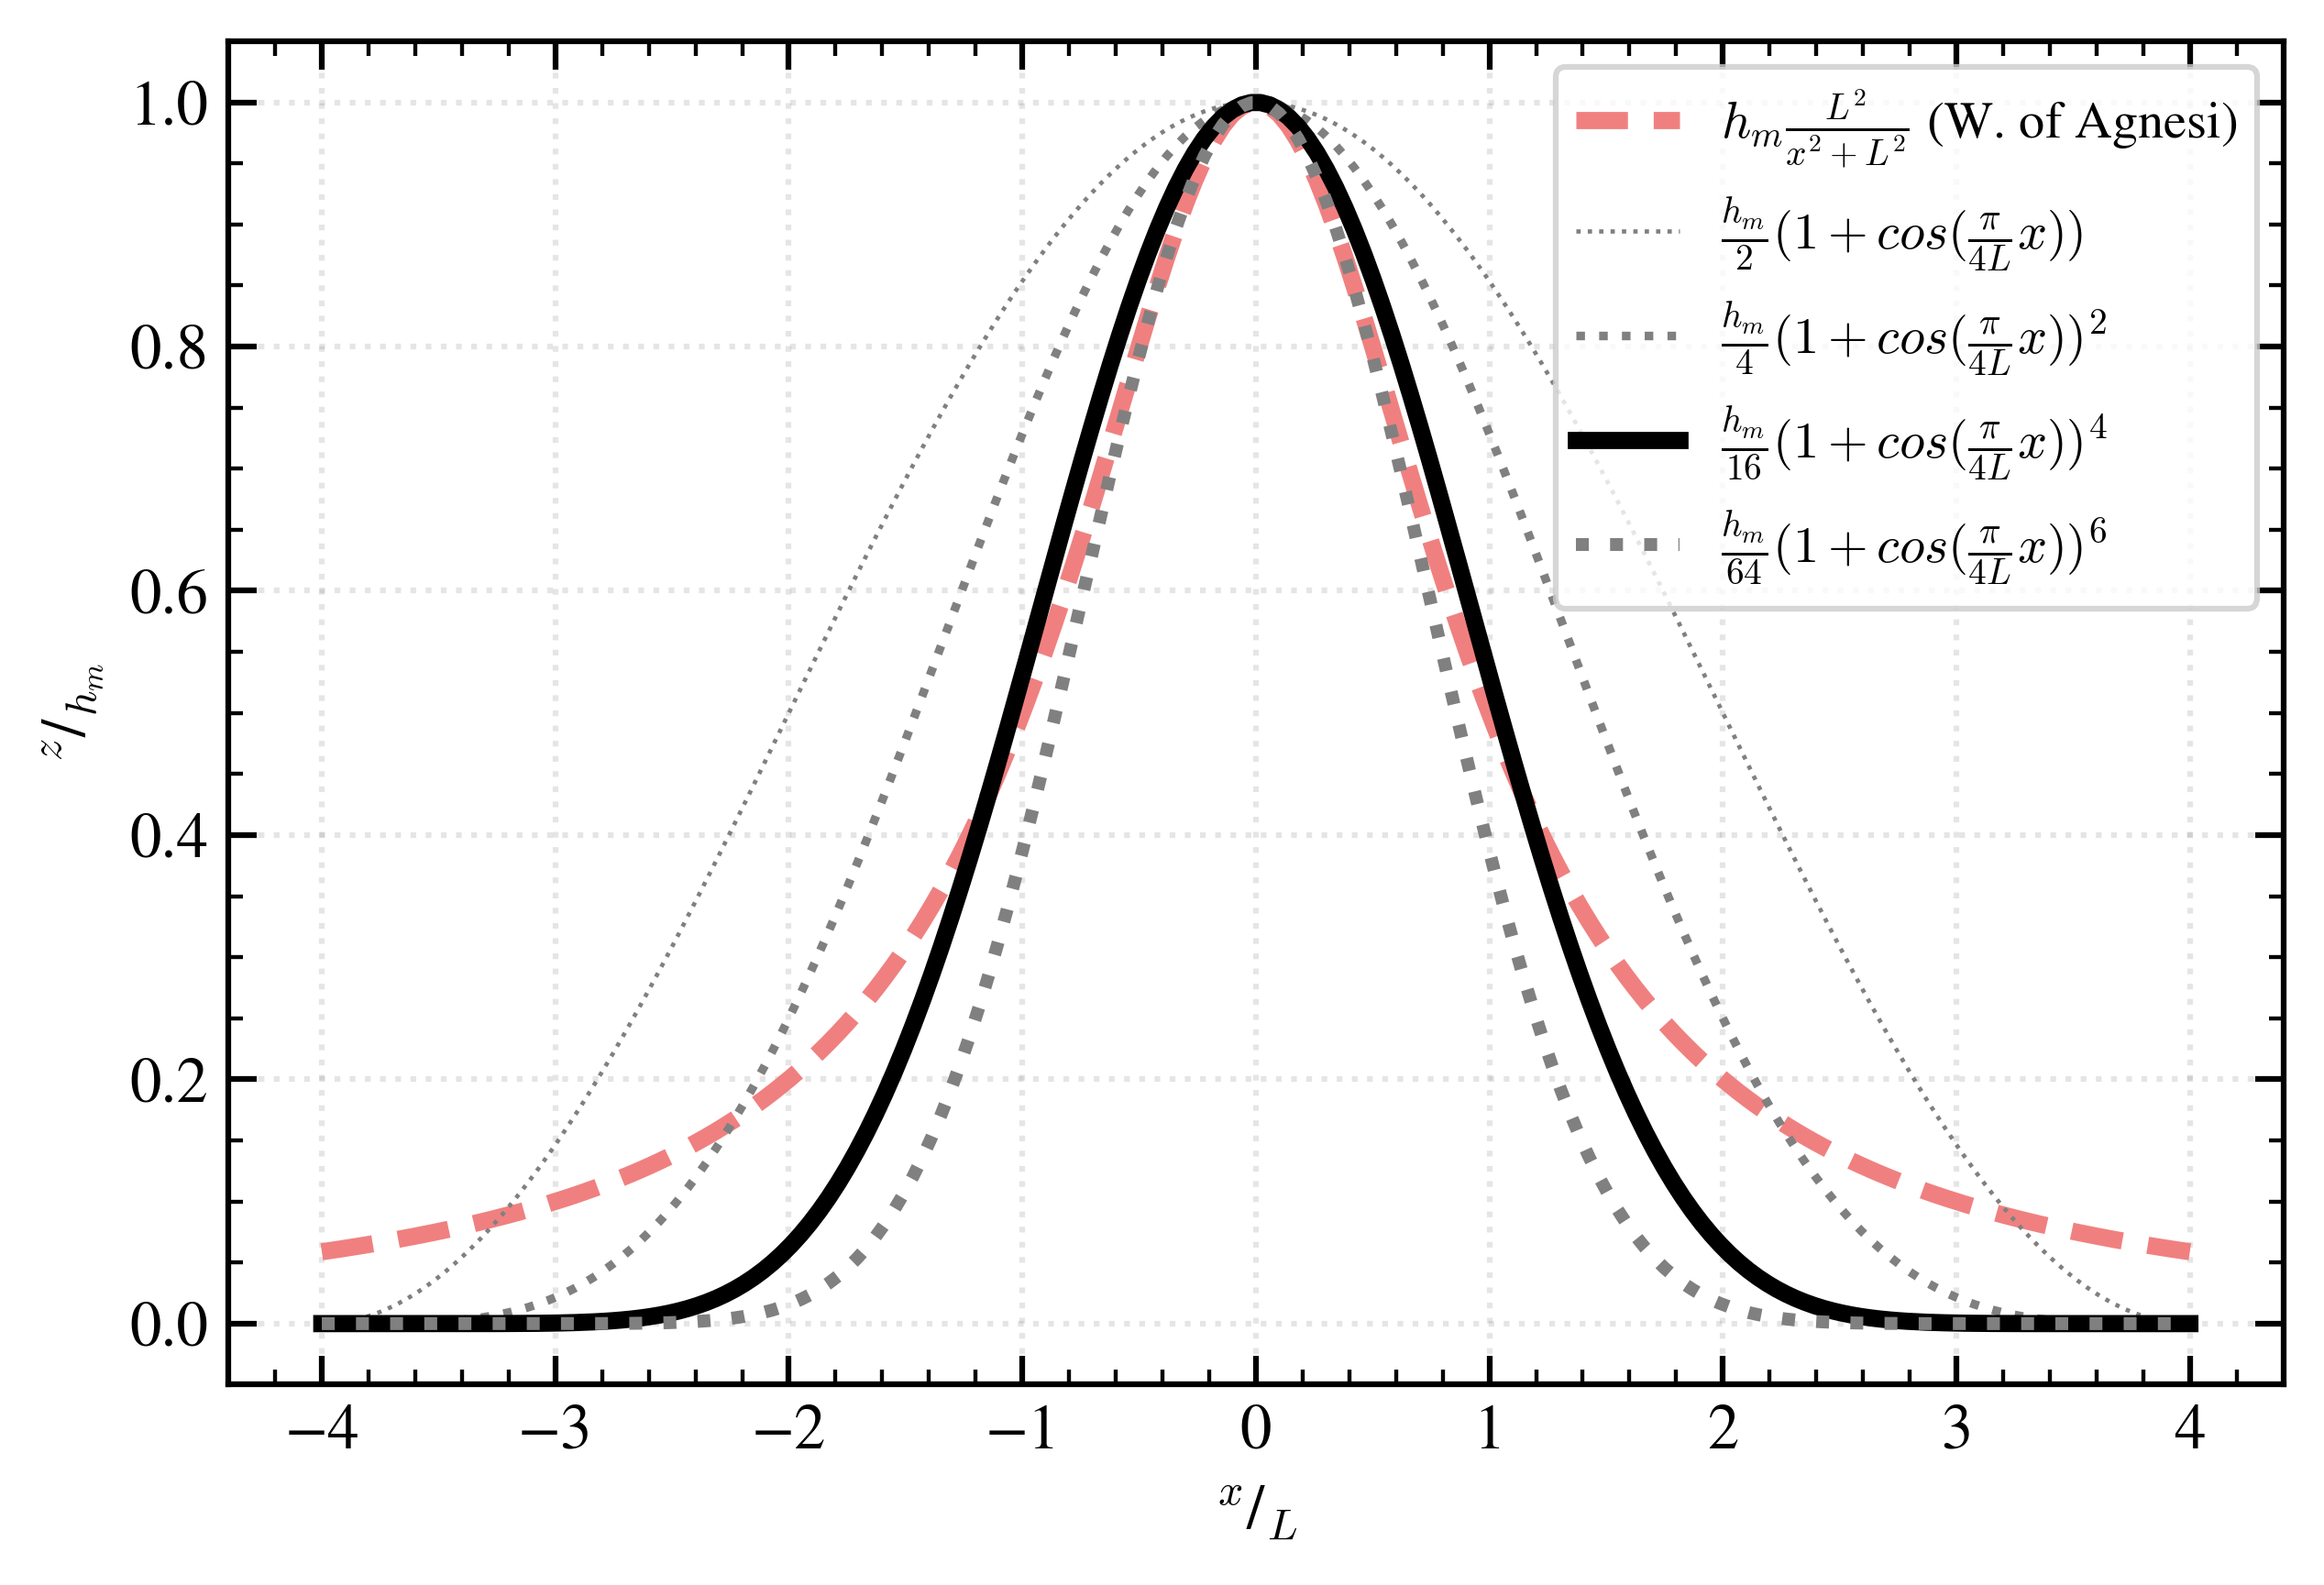
\includegraphics[width=0.67\textwidth]{figures_model/topo-transient-boundary.png}
    \caption{Shown are different variations of a $(1+cos(x))$ mountain (black solid and dotted lines) and a Witch of Agnesi (red dashed line). The vertical dimension is scaled by the mountain height $h_m$, the horizontal dimension by the mountain half width $L$. It allows a comparison of all shapes independent of $h_m$ and $L$.}
    \label{fig:topo_trans}
\end{figure*} 

In EULAG the transient surface boundary \code{zs} is defined within the subroutine \code{topol\_vert()}. \code{zs} and its time derivative \code{zsd} have to be continuous, so \code{zs} has to be differentiable. The following set of equations describe the time-dependent 2D surface \code{zs(tt,y,x)} for a 3D simulation of chapter \ref{sec:results3D} with an elliptical tropopause depression. Derivatives are left out and it should be noted that the equations vary for the elongated ridge (compare Figure \ref{fig:q3D_referenceSim}) in chapter \ref{sec:resultsQ3D}.
\begin{equation}
    \code{zs(tt,y,x)} = h_{cos}(\code{rr}) =\frac{1}{16} \bigl(1+cos(\frac{\pi}{4} \code{rr})\bigr)^4
    \label{equ:cosMtn-1}
\end{equation}
\begin{equation}
    \code{rr} = \sqrt{\bigl(\frac{\code{xx}}{\code{xml}}\bigr)^2 + \bigl(\frac{\code{yy}}{\code{yml}}\bigr)^2}
    \label{equ:cosMtn-2}
\end{equation}
\begin{equation}
    \begin{aligned}
        \code{xx} &= \code{cang}(\code{x}-\code{x0}) + \code{sang}(\code{y}-\code{y0}) \\
        \code{yy} &=-\code{sang}(\code{x}-\code{x0}) + \code{cang}(\code{y}-\code{y0}) 
    \end{aligned}
    \label{equ:cosMtn-3}
\end{equation}
\begin{equation}
    \begin{aligned}
    \code{x0} &= \code{x00} + \code{ctopo} \cdot \code{tt} \\ 
    \code{y0} &= \code{y00} = 0
    \label{equ:cosMtn-4}
    \end{aligned}
\end{equation}
with \code{xml} and \code{yml} being the width of the tropopause fold in zonal and meridional direction, \code{cang}=cos(\code{ang}) and \code{sang}=sin(\code{ang}) with \code{ang} being the angle of the fold's axes with respect to the domain axes. \code{ang} is used for rotating the tropopause fold in chapter \ref{sec:results3D}. \code{x00} and \code{y00} refer to the initial location of the fold's center and $\code{ctopo}=c_{tf}=\SI{13.88}{\meter \per \second}$ defines the propagation speed of the fold.

Another usecase of a time-dependent boundary or surface of the simulation is the initialization process. Idealized simulations with a surface topography start with a flat surface and homogeneous horizontal flow instead of initialising the flow field with a potential flow. Then the topography slowly grows for a defined time \code{tspinup}. In EULAG the surface \code{zs} is multiplied by
\begin{equation}
    \code{tf}(t) = t^3 (10 - 15t + 6t^2)
    % \code{tf}(\frac{\code{tt}}{\code{tspinup}}) = \Bigl(\frac{\code{tt}}{\code{tspinup}}\Bigr)^3 \biggl(10 - 15 \frac{\code{tt}}{\code{tspinup}} + 6 \Bigl(\frac{\code{tt}}{\code{tspinup}}\Bigr)^2\biggr)
    \label{equ:spin-up}
\end{equation}
with $t = \code{tt} / \code{tspinup}$ for $\code{tt} < \code{tspinup}$. The time derivative \code{zsd} is modified accordingly. \\
We use equation \ref{equ:spin-up} with $\code{tspinup}=\SI{12}{\hour}$ for a growing tropopause fold in all simulations. A wind ramping that slowly increases the surface wind to its stationary value can be an alternative strategy to circumvent unphysical processes during the initialization (e.g. \cite[]{mixa_nonlinear_2021}), but it is not used in the presented simulations.
% $c_{tf}$=\SI{13.88}{\meter \per \second} 

\section{Non-linear simulations of MW regimes with linear analytic solutions}
\label{sec:linear-MWs}
Though EULAG has proven itself to be a reliable tool for simulating a wide range of flows and specifically atmospheric flows over steep terrain (\cite{prusa_eulag_2008} and \cite{doyle_intercomparison_2011}) this section validates our specific model setup for simulating propagating tropopause folds. In a first step, we conducted simulations of a 'moving' mountain in a quiescent fluid (no background wind) and compared the propagation of GWs to our predictions from linear theory. In addition, we reproduced the 2D simulations of \textcite[]{prusa_all-scale_2003} with an oscillating tropopause fold at the lower boundary to confirm a correct implementation of the time-dependent boundary. We do not show these results and refer to the work of \textcite{grogger_simulation_2022} for further interesting experiments and tests with the EULAG model in general and specifically for transient boundary conditions. We focus instead on the comparison of non-linear model results from EULAG to analytic solutions of linear GW theory. 

The assumption of an impermeable tropopause at the lower boundary of the numerical simulations makes a tropopause depression act like an upside down mountain (valley) on the stratospheric flow above. In that sense, it is the goal to reproduce some fundamental analytic results of different MW regimes (non-hydrostatic GWs, hydrostatic GWs, inertia-gravity waves (IGWs)) with the EULAG model. \textcite{queney_problem_1948} was the first to derive linear solutions of the flow field for these different regimes assuming only small adiabatic perturbations. Many studies followed and contributed to a collection of analytic solutions for a wide range of scenarios. For the simplified cases of \textcite{queney_problem_1948} with a Witch of Agnesi mountain, constant background flow $U$ and stratification $N$ even solutions for the total gravity wave drag (GWD) exist, which can also be computed in numerical simulations (\cite[]{teixeira_physics_2014}). This makes the GWD a useful parameter to validate a numerical model with an analytic reference. Solutions are available for the whole range of mountain half widths $L$ and a concise summary on this topic is found in section 8.8 and Figure 8.10 in \textcite{gill_atmosphere-ocean_1982}. We will reproduce and discuss Figure 8.10 from \textcite[]{gill_atmosphere-ocean_1982} together with our model results and more recent theoretical studies in the next subsection. Subsequently, we continue with an interpretation of simulation based vertical profiles of momentum and energy fluxes, because they nicely illustrate various aspects in the context of momentum and energy conservation and the Eliassen-Palm (EP) relation. But first, we outline the numerical simulations of different MW regimes.

All simulations prescribe a Witch of Agnesi topography (equation (\ref{equ:agnesi})) with a small amplitude $h_m = \SI{100}{\meter}$ to minimize non-linear effects. Nine different mountain half widths from $L = 1-\SI{150}{\kilo\meter}$ are considered to cover the whole range of MW scenarios from non-hydrostatic GWs (high frequency waves) and hydrostatic GWs (medium frequency waves) to IGWs (low frequency waves). Ambient profiles follow the isothermal Bacmeister-Schoeberl model from section \ref{sec:ambient-profiles} with parameters for the troposphere (first column of table \ref{tab:ambientProfiles}). Therefore, $N=\SI{0.01}{\per\second}$ and the Coriolis frequency $f = 0.01 N = \SI{1e-4}{\per\second}$ (refers to a latitude of $\approx \SI{45}{\degree}$) and $u_e =\SI{10}{\meter\per\second}$ to be consistent with the analytic solutions in \textcite[]{queney_problem_1948} and \textcite[]{gill_atmosphere-ocean_1982}. \\
The horizontal domain and resolution varies between simulations, while the vertical dimension (z$_{top}=\SI{35}{\kilo\meter}$) and resolution ($\Delta$z$=\SI{50}{\meter}$) is fixed. The temporal resolution decreases for larger $L$ to reach a stationary state with the same amount of timesteps. All simulations simulate $n_t$=\SI{5760}{timesteps} on a grid with (n$_z$,n$_y$,n$_x$)=(701,48,960) grid points. Different resolutions are summarized in table \ref{tab:linearRegimes} which also provides relevant settings for vertical and horizontal sponge layers. These also change between simulations to ensure a smooth dissipation of wave energy and minimize wave reflection. \\
%
\begin{table*}[t]
    \centering
    \caption{Parameters for numerical simulations of different MW regimes: mountain width $L$, spatial increments $\Delta$x, $\Delta$y and $\Delta$z in the horizontal and vertical directions, time step $\Delta$t and the corresponding Courant-Friedrichs-Lewy (CFL) condition, thickness $\delta$x$_{ab}$ and time scale $\tau_x$ of the horizontal and altitude z$_{ab}$ and time scale $\tau_z$ of the vertical absorbers.}
    \begin{tabular}{@{}cccccccccc@{}}
    \toprule
    $L$/km & $\Delta$x/m & $\Delta$y/m & $\Delta$z/m & $\Delta$t/s & CFL/- & $\delta$x$_{ab}$/km & $\tau_x$/s  & z$_{ab}$/km & $\tau_z$/s \\ \midrule[1pt]
    1   & 50 & 2000 & 50 & 5 & 1 & 15  & 300  & 24 & 300   \\
    2   & 100 & 2000 & 50 & 5 & 0.5  & 30  & 600  & 24 & 450   \\
    5   & 250 & 5000 & 50 & 10 & 0.4 & 75  & 1200 & 24 & 600  \\
    10  & 500 & 10000 & 50 & 20 & 0.4  & 100 & 1800 & 24 & 900  \\
    25  & 1000 & 50000 & 50 & 40 & 0.4  & 200 & 3600 & 24 & 2400  \\
    50  & 1500 & 50000 & 50 & 60 & 0.4  & 300 & 4500 & 24 & 5400  \\
    75  & 2000 & 100000 & 50 & 60 & 0.3 & 400 & 6000 & 24 & 10500 \\
    100 & 2500 & 100000 & 50 & 75 & 0.3  & 500 & 7500 & 24 & 12000 \\
    150 & 3500 & 100000 & 50 & 180 & 0.51 & 700 & 9000 & 24 & 21000 \\
    \bottomrule
    \end{tabular}
    \label{tab:linearRegimes}
\end{table*}
The simulation for $L=\SI{100}{\kilo\meter}$ is shown in Figure \ref{fig:MWs-reference} with a vertical (a) and a horizontal (b) cross section after t$=\SI{120}{\hour}$. As expected for this large mountain width, IGWs propagate upward and into the lee of the mountain where they dissipate due to the sponge layers. Linear sponge or absorber layers are chosen quite thick to allow larger dissipation timescales $\tau$. Since $\Tilde{\alpha}$ and $\Tilde{\beta}$ in equations (\ref{equ:momEqu}) and (\ref{equ:potTemp}) of the anelastic framework are inverse proportional to $\tau$ (equation (\ref{equ:linear-sponge})) larger timescales $\tau$ reduce local forcings related to the damping and minimize wave reflection at the sponge interfaces and the model top. The meridional extent is very large to minimize any impacts of the ridge ends on the zonal cross section at y$=\SI{0}{\kilo\meter}$ that is used for the following analysis (calculating the total GWD and zonal averages of vertical profiles).
\begin{figure*}[t]
    \centering
    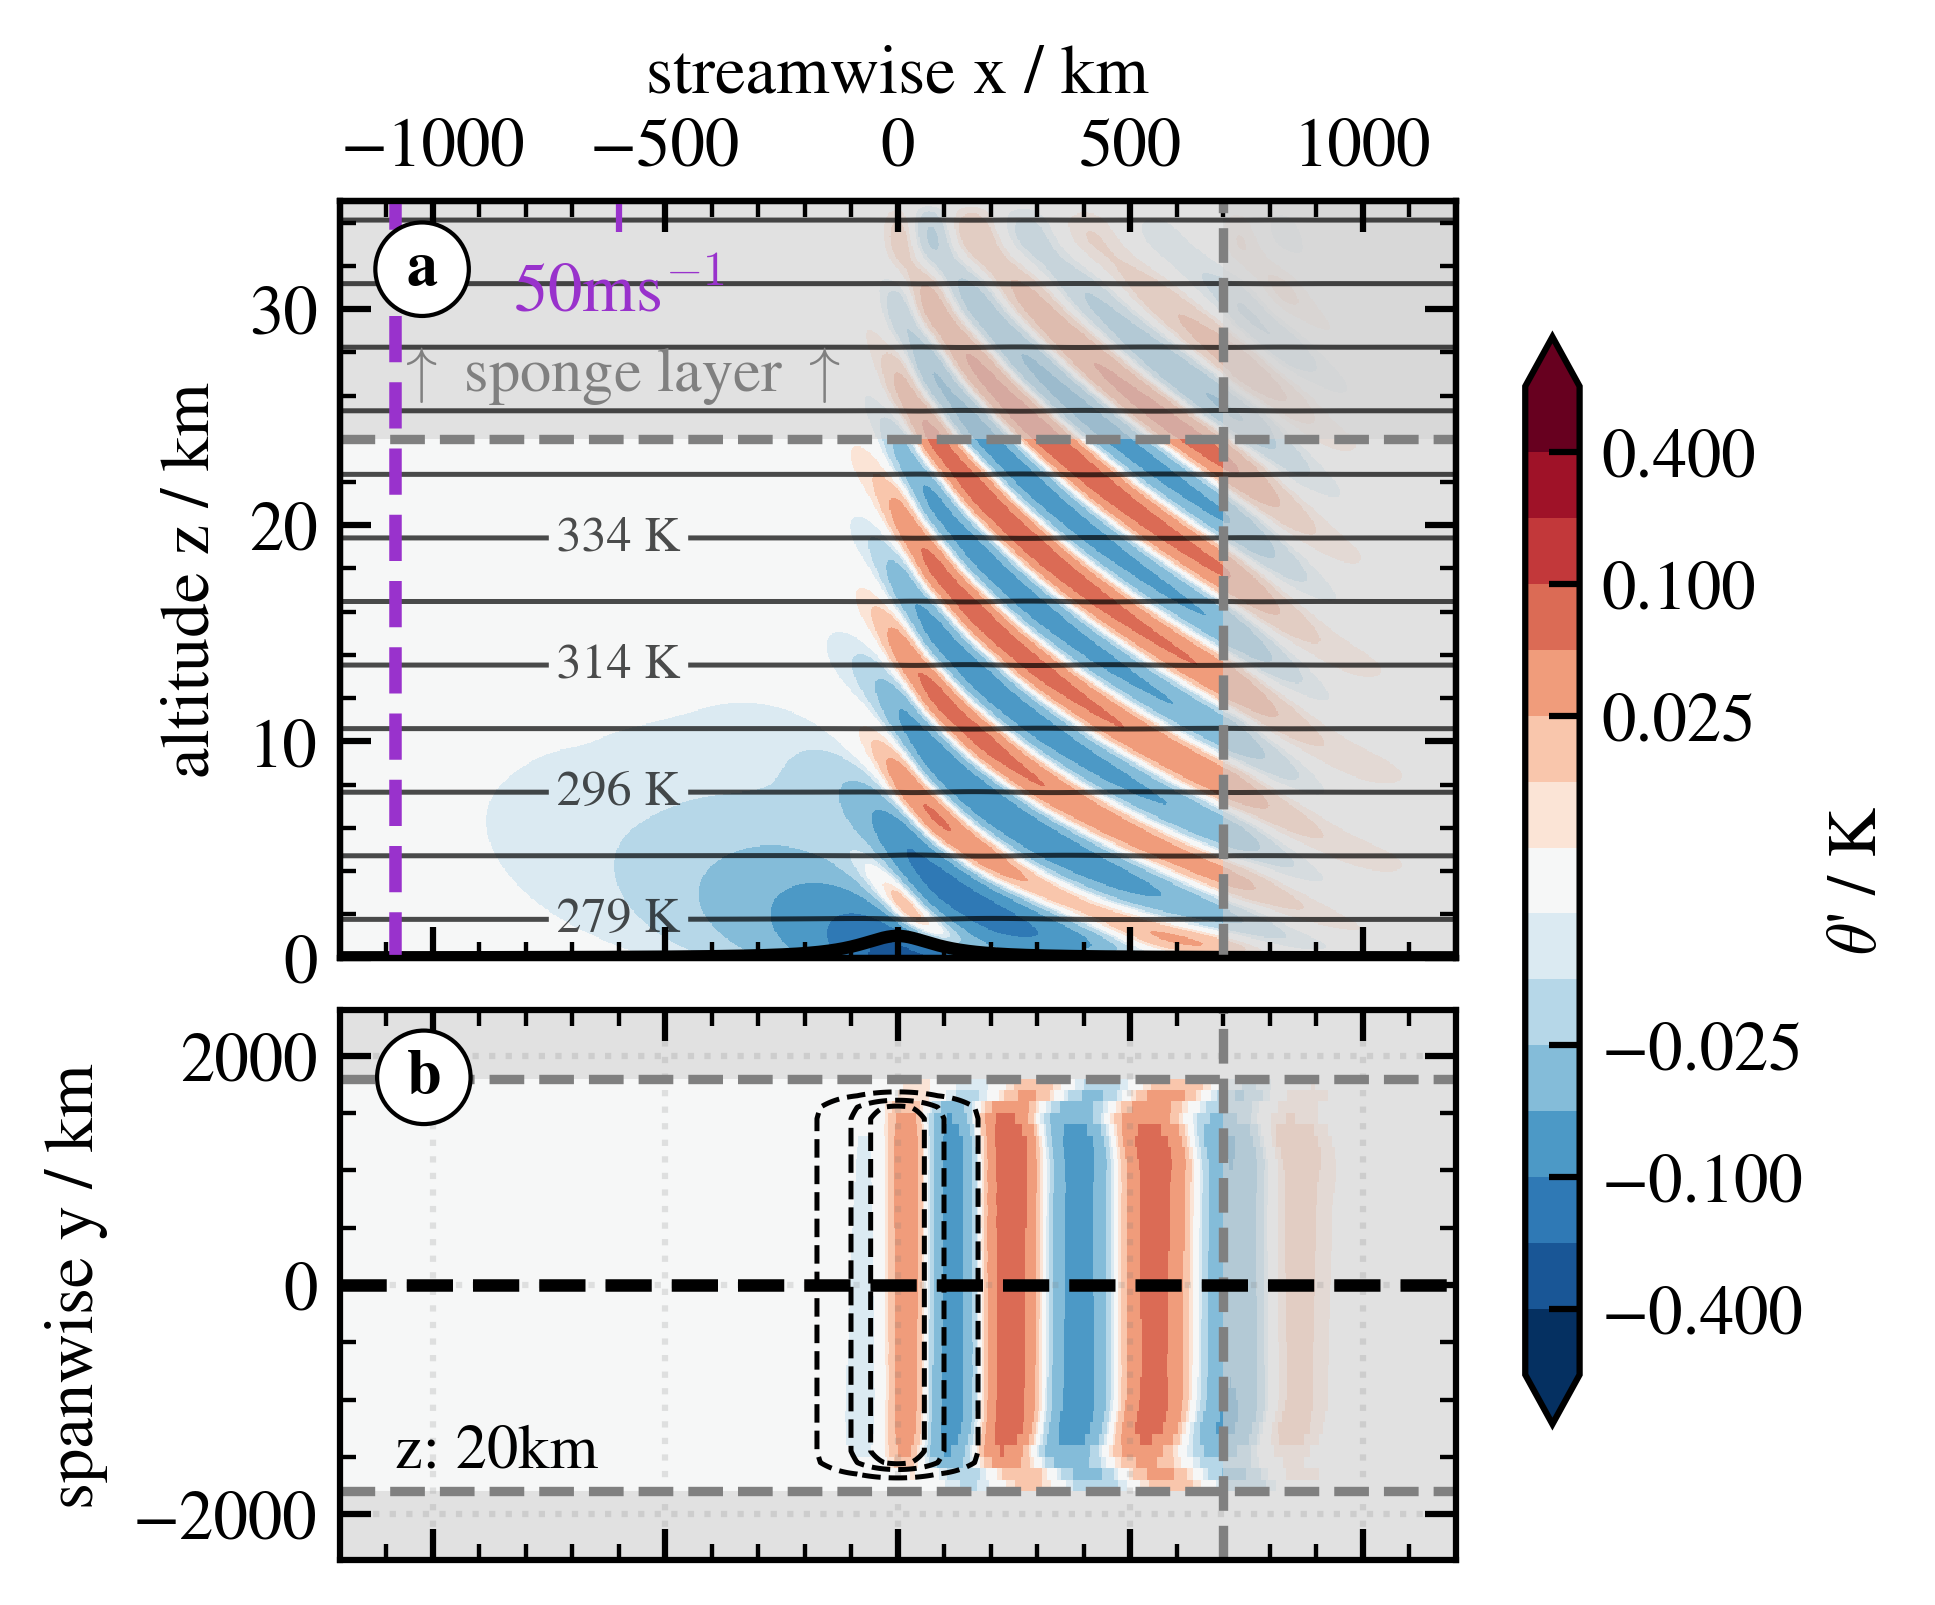
\includegraphics[width=0.67\textwidth]{figures_model/MWs-th-referenceSim.png}
    \caption{Centered vertical cross section (a) and horizontal cross section at z$=\SI{20}{\kilo\meter}$ (b) of potential temperature perturbations $\Theta'$ for a mountain width $L=\SI{100}{\kilo\meter}$ after t$=\SI{120}{\hour}$. Grey areas represent sponge layers (upstream sponge layer not shown) and the purple dashed line in (a) shows the constant wind profile with U$=\SI{10}{\meter\per\second}$. The thick dashed black line in (b) marks the relevant cross section for further analysis. The surface topography is exaggered by a factor of 10 and it should be noted that axes of (b) are not to scale.}
    \label{fig:MWs-reference}
\end{figure*}

% .􏰝α and β􏰝 are zero everywhere, except in the vicinity of the vertical and lateral boundaries where they increase linearly to one towards the model boundaries.
% courant number fulfilled?? 
% Wentzel-Kramers-Brillouin WHB method or approximation
% To be concise
%%%%%%%%%%%%%%%% GWD %%%%%%%%%%%%%%%%%
\subsection*{Gravity wave drag and angular momentum flux}
MW scenarios imply that an asymmetry in the pressure distribution across the mountain develops. Consequently, the atmosphere exerts a force on the orography that tends to accelerate the topography in the direction of the mean flow. This force  
\begin{equation}
    F_{GWD} = F_x = \int_{-\infty}^{\infty} p' \frac{\partial h}{\partial x} dx
    \label{equ:gwd}
\end{equation}
is called pressure drag and in the case of GWs it is also called gravity wave drag (GWD) (e.g. \cite[]{gill_atmosphere-ocean_1982} or \cite[]{durran_lee_2003}). Theoretical linear solutions for the GWD as a function of the mountain width exist for the whole spectrum of MWs assuming a steady state and only small adiabatic perturbations. While \textcite[]{blumen_momentum_1965} derived a solution for the high frequency spectrum (non-hydrostatic GWs), \textcite[]{smith_influence_1979} presented one for low frequency waves (IGWs). Both are based on Bessel functions and have been combined in Figure 8.10 of \textcite[]{gill_atmosphere-ocean_1982} to present a non-dimensional solution for the GWD for the whole range of mountain widths. Figure \ref{fig:GWD-MWs} also shows these solutions superimposed by results from our non-linear numerical simulations with the EULAG model and a more recent analytic solution from linear theory for the hydrostatic rotating limit. This alternative solution from \textcite{miranda_non-linear_1992} represented by the orange line in Figure \ref{fig:GWD-MWs} suggests a higher GWD for large mountain widths. Apparently, values from our non-linear simulations align with their results and not with the solution of \textcite[]{smith_influence_1979}. Is this plausible? \\
Smith's solution follows Queney's and assumes a steady flow that is independent of the y coordinate for the linearized Boussinesq equations of a rotating stratified fluid. In this case, independent of the y coordinate implies an infinite ridge shape and no pressure gradient in meridional direction in the momentum equation ($\frac{\partial p}{\partial y}=0$). The approach of \textcite[]{miranda_non-linear_1992} also uses the linearized Boussinesq equations for a rotating stratified fluid, but it allows $\frac{\partial p}{\partial y}\neq 0$ and keeps the 3D shape of a circular bell-shaped mountain as introduced by \textcite[]{smith_linear_1980} and \textcite[]{phillips_analytical_1984}. Instead, they assume zero meridional wind ($V=0$), integrate over two dimensions and end up with 
\begin{equation}
    F_{GWD} = \int_{-\infty}^{\infty} \int_{-\infty}^{\infty} p' \nabla h \, dx \, dy = \frac{\pi}{4} \rho_0 N U L h_0^2 \Bigl( \bigl(1 + \frac{2fL}{U}\bigr) e^{-\frac{2fL}{U}} \Bigr)
    \label{equ:gwd-miranda}
\end{equation}
for the hydrostatic rotating limit of a circular bell-shaped mountain. Though they define a circular mountain, the combination with $V=0$ seems to form a framework for linear solutions that match the numerical simulations with an elongated ridge. GWD values that result from non-linear simulations of a circular mountain are significantly lower.
 \begin{figure*}[t]
    \centering
    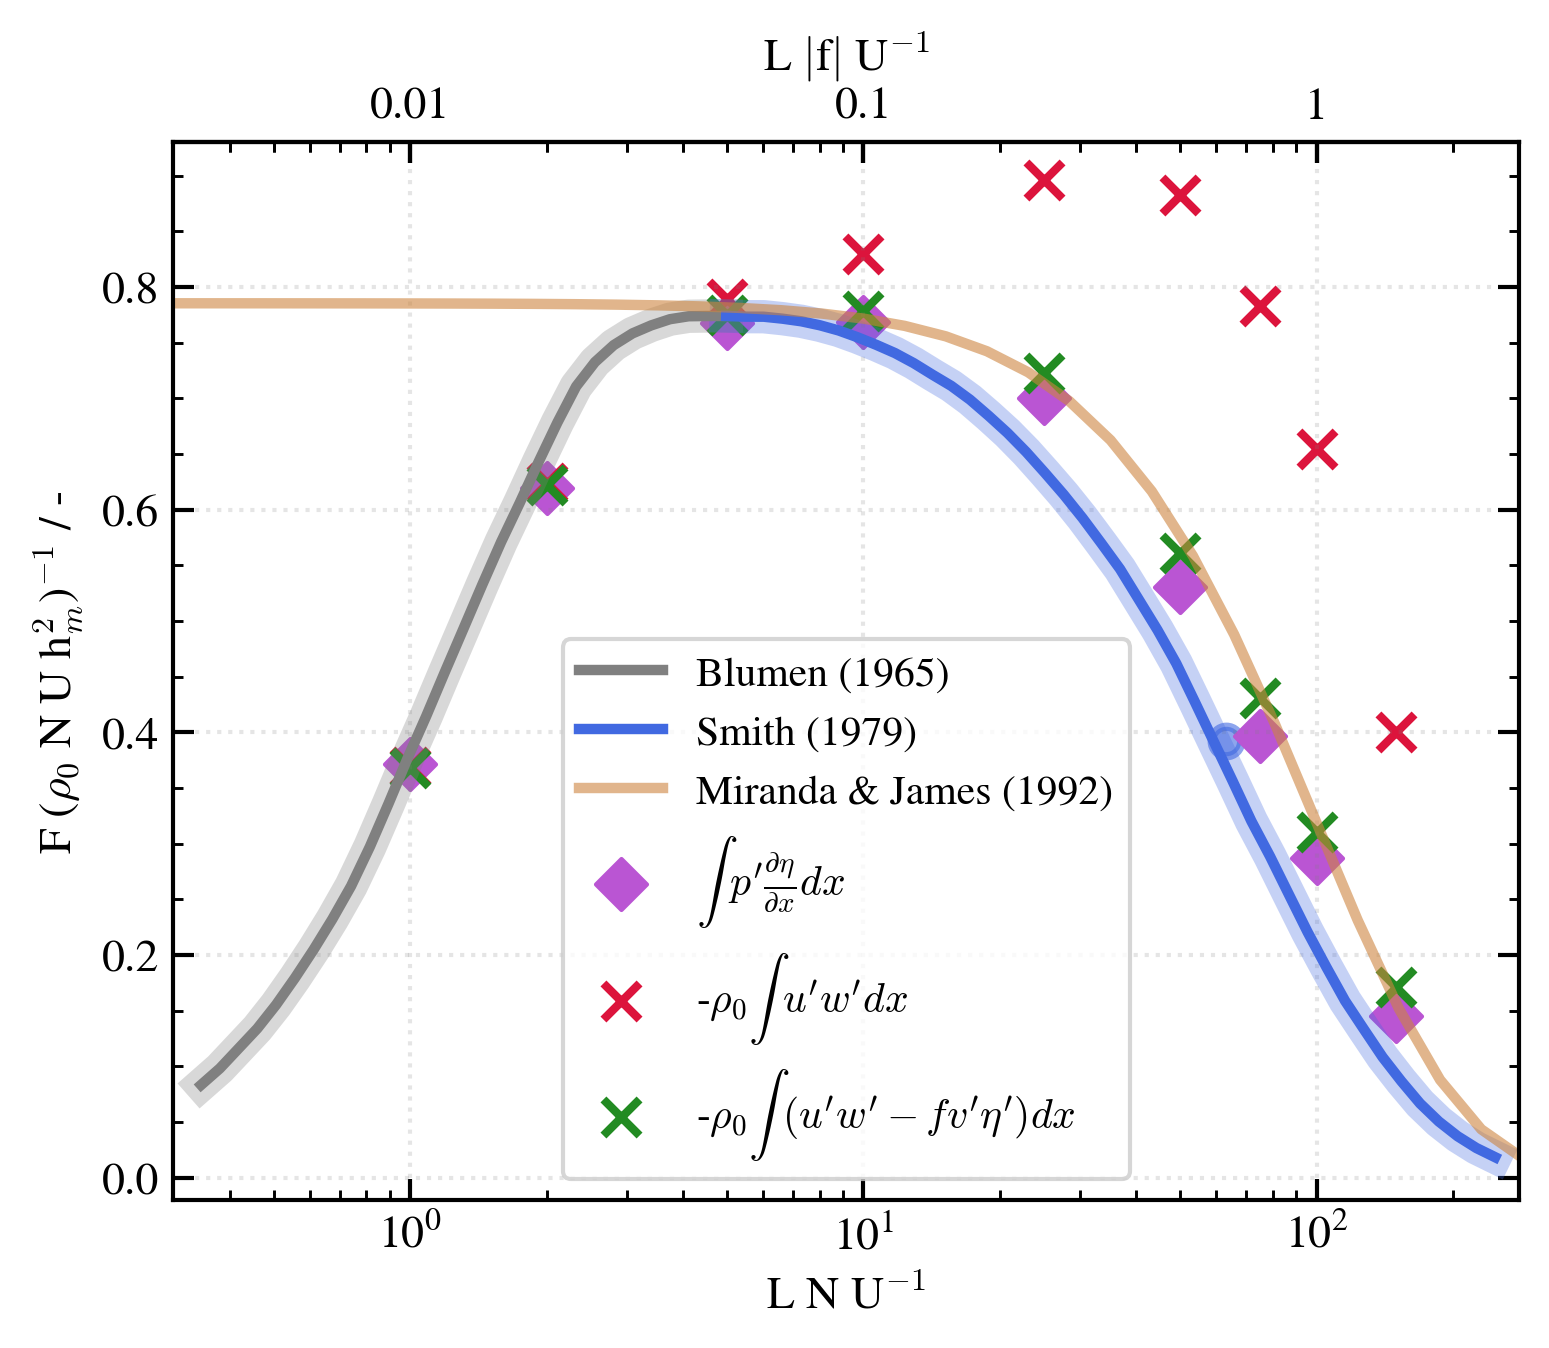
\includegraphics[width=0.63\textwidth]{figures_model/GWD-linearTheory-Q3D.png}
    \caption{The force $F$ is the GWD $F_x$ normalized by $\rho_0 \textrm{N} \textrm{U} \textrm{h}_m^2$ for the linear momentum flux of the flow over a Witch of Agnesi with half width $L$. Thicker faded lines indicate that the linear solution is based on Bessel functions (\cite[]{blumen_momentum_1965} and \cite[]{smith_influence_1979}). \textcite[]{miranda_non-linear_1992} provide an analytical solution for the hydrostatic rotating limit (IGWs). Buoyancy frequency N and flow speed U are uniform and the Coriolis frequency $f=0.01$N. Purple hashes represent the GWD or pressure drag, red crosses the linear momentum flux MF$_x$ and green crosses the angular momentum flux MF$_{x,ang}$ as described in \textcite[]{bretherton_momentum_1969}, \textcite[]{smith_influence_1979} and \textcite[]{broad_linear_1995} for different MW simulations with varying mountain half width $L$.}
    \label{fig:GWD-MWs}
\end{figure*}

Different values from the numerical simulations are plotted to emphasize the effect of rotation on the GWD. For a non-rotating fluid the vertical flux of horizontal momentum (for turbulent motion also called the Reynolds stress)
\begin{equation}
    (\mathrm{MF}_x, \mathrm{MF}_y) = \bar{\rho}  (\overbar{u'w'},\overbar{v'w'})
    \label{equ:mf}
\end{equation}
with the overbar denoting an average over one or multiple full wave cycles can be related to the GWD. Modifying the zonal momentum equation with the continuity equation, integrating throughout the volume from the surface $h(x)$ to an arbitrary height $z_t$ and considering that there is no advective momentum flux through the lower boundary yields
\begin{equation}
    \frac{\partial}{\partial t}\int_{}^{} \int_{}^{} \int_{}^{} \rho u' dV = - \left.\int_{}^{} \int_{}^{} \rho u'w' \, dx \, dy \right\vert_{z=z_t}  \,
    - \left.\int_{}^{} \int_{}^{} p' \frac{\partial h}{\partial x} \, dx \, dy \right\vert_{z=h}
    \label{equ:gwd-mf}
\end{equation}
and for a steady-state flow
\begin{equation}
    \left.\int_{}^{} \int_{}^{} p' \frac{\partial h}{\partial x} \, dx \, dy \right\vert_{z=h} =  -\left.\int_{}^{}  \int_{}^{} \rho u'w' \, dx \, dy \right\vert_{z=z_t}
    \label{equ:gwd-mf-2}
\end{equation}
the pressure drag equals the negative momentum flux (e.g. \cite[]{durran_lee_2003}). In other words, a positive pressure drag is compensated by a negative (downward) flux of horizontal momentum. \\
The negative zonal momentum flux MF$_x$ from equation (\ref{equ:mf}) is represented by the red crosses in Figure \ref{fig:GWD-MWs}. For smaller mountain widths up to $L=\SI{5}{\kilo\meter}$ it is more or less identical to the pressure drag (purple hashes), but starts to deviate as soon as rotational effects become important. \textcite[]{bretherton_momentum_1969} nicely illustrated why equation (\ref{equ:gwd-mf-2}) is not valid anymore for rotating fluids though MF$_x$ is still the momentum transfer across a flat horizontal surface (z$=$const.). He starts from the linearized momentum equation for a rotating fluid in the Boussinesq approximation
\begin{equation}
    U \frac{\partial u'}{\partial x} + w' \frac{\partial U}{\partial z} - f v' = -\frac{1}{\rho} \frac{\partial p'}{\partial x}
    \label{equ:momEqu-rotating}
\end{equation}
and notes that the pressure drag (equation (\ref{equ:gwd})) can be rewritten for the horizontal force across the wavy (not horizontal) surface z$= \eta(x)=h(x)$ to
\begin{equation}
    F_x =  \int_{-\inf}^{\inf} p' \frac{\partial \eta}{\partial x} dx = -\int_{-\inf}^{\inf} \eta' \frac{\partial p'}{\partial x} dx
    \label{equ:pdrag-rotating}
\end{equation}
by applying integration by parts. We follow the notation of \textcite[]{smith_influence_1979} or \textcite{broad_linear_1995} and use $\eta$ for the vertical and not the meridional displacement. Equation (\ref{equ:momEqu-rotating}) becomes 
\begin{equation}
    F_x =  -\int_{}^{} \rho u' \Bigl(U \frac{\partial \eta}{\partial x}\Bigr) \, dx + \rho \frac{\partial U}{\partial z} \int_{}^{} w' \eta' \, dx  - f \int_{}^{} \rho v' \eta' \, dx 
    \label{equ:momEqu-rotating-2}
\end{equation}
and after linearizing with $w'=U\frac{\partial \eta}{\partial x}$ the second term vanishes and
\begin{equation}
    F_x = \mathrm{MF}_{x,ang} = -\int_{}^{} \rho u'w' \, dx  -  \int_{}^{} \rho f v' \eta' \, dx
    \label{equ:angular_momentum}
\end{equation}
with a first term representing the vertical flux of linear momentum MF$_x$ and a second term that represents the Coriolis force acting in the region between the undisturbed, leveled streamline and the vertically displaced streamline. For rotating fluids it is equation (\ref{equ:angular_momentum}) that is equal to the pressure drag of equation (\ref{equ:gwd}). It is called the vertical flux of angular momentum and can be interpreted as the force exerted across a surface always consisting of the same material particles (Lagrangian perspective) that differs from the linear momentum across a horizontal plane (Eulerian perspective) by the Coriolis term in equation (\ref{equ:angular_momentum}). \\
In Figure \ref{fig:GWD-MWs} the angular momentum is represented by the green crosses. It is slightly higher than the pressure drag for larger mountain widths, but the difference is small. It was checked if compressible effects can explain this difference considering the compressible solution of the GWD from linear theory 
\begin{equation}
    F_x =  \rho_0 \int_{}^{} (u'w' + f v' \eta') \, dx + f \int_{}^{} \rho' v' \eta' \, dx
    \label{equ:angular_momentum_compressible}
\end{equation}
derived by \textcite[]{broad_linear_1995}. Dropping the Boussinesq approximation adds another term to the streamwise GWD involving density fluctuations. However, the normalized contribution of the compressible part $f \rho' v' \eta'$ in equation (\ref{equ:angular_momentum_compressible}) was at maximum $\mathcal{O}(10^{-5})$ and can not explain the difference between the pressure drag and the angular momentum in Figure \ref{fig:GWD-MWs}. It is not fully understood what causes this inconsistency of the pressure drag, but theories exist and will be discussed in the context of vertical profiles in the next subsection. 

Overall, GWD values from non-linear simulations with EULAG successfully reproduce analytic solutions of the GWD from linear theory for the whole range of MWs from non-hydrostatic GWs to IGWs. In particular, the surface angular momentum MF$_{x,ang}$ closely follows the linear solution of \textcite[]{miranda_non-linear_1992} for the hydrostatic rotating limit.

% Though $V=0$, 3D critical layers might be relevant for the 3D flow of IGWs with increasing meridional perturbations $v'$ for larger mountain widths as discussed in section \ref{sec:q3D-wind}. but vertical profiles in next section suggest that all simulations obey linear wave propagation... from EP relation. 

% ecause in plane inertio-gravitational waves a vertical displacement 5 is correlated with a Ox displacement ( and hence with an Oy velocity v, these contributions are systematically of one

% \cite[]{jones_propagation_1967} was first before bretherton 
% \cite[]{teixeira_physics_2014}
% gaussian quadrature 
% dimensionless drag is specified differently for Smith and miranda due to additional dimension

% Geostrophic balance: fu = - 1/rho * dp/dy
% f negative for southern hemisphere but not for idealized simulations of MWs
% possible to run EULAG simulation with meridional gradient of p?
% Are results interesting for further investigation of ini probs? I guess this geostrophic balance develops but can we filter out its contribution to p'?

%%%%%%%%%%%%%%%% VERTICAL PROFILES %%%%%%%%%%%%%%%%%
\subsection*{Vertical profiles of momentum and energy fluxes}
For linear, non-rotating (2D), steady-state flows equation (\ref{equ:gwd-mf-2}) is valid for any upper level $z_t$, so the linear momentum is conserved in the vertical as long as U$\neq 0$ (\cite[]{durran_lee_2003}). In their seminal work \textcite[]{eliassen_transfer_1960} present a consistent result relating the linear momentum flux to the gradient of the vertical flux of wave energy EF$_z = \overbar{p'w'}$
\begin{equation}
    -\frac{\partial}{\partial z}\overbar{p'w'} = \frac{\partial U}{\partial z} \cdot \bar{\rho} \overbar{u'w'}
    \label{equ:EP-relation-dudz}
\end{equation}
and to EF$_z$ directly
\begin{equation}
    \begin{aligned}
    -\overbar{p'w'}& = U \cdot \overbar{u'w'} \\
    -\mathrm{EF}_z& = U \cdot \mathrm{MF}_x.
    \end{aligned}
    \label{equ:EP-relation}
\end{equation}
Equation (\ref{equ:EP-relation}) is called the Eliassen-Palm (EP) relation and is valid for linear, steady, small-amplitude, non-dissipative wave propagation. Under these assumptions, equation (\ref{equ:EP-relation-dudz}) and (\ref{equ:EP-relation}) again state that the vertical flux of horizontal momentum is conserved in the vertical and that EF$_z$ changes in proportion to the gradient of $U(z)$. For $U(z)=$const. EF$_z$ does not change with height, too.

\textcite[]{broad_linear_1995} combined the analysis methods of \textcite[]{eliassen_transfer_1960} and \textcite[]{bretherton_momentum_1969} to obtain a similar set of equations for the general case of a 3D rotating fluid. Modifying the 3D energy equation according to \textcite[]{eliassen_transfer_1960} provides 
\begin{equation}
    -\frac{\partial}{\partial z} \mathrm{EF}_z = \frac{\partial U}{\partial z} \cdot \mathrm{MF}_{x,ang} + \frac{\partial V}{\partial z} \cdot \mathrm{MF}_{y,ang}
    % U(z) \cdot \frac{d}{dz}\mathrm{MF}_{x,ang} + V(z) \cdot \frac{d}{dz}\mathrm{MF}_{y,ang} = 0
    \label{equ:EP-relation-rotating-dudz}
\end{equation}
and considering the horizontal momentum across the wave surface $z=\eta(x,y)$ (not the horizontal surface) according to \textcite[]{bretherton_momentum_1969} yields
\begin{equation}
    \begin{aligned}
        -\overbar{p'w'}& = U \cdot \bar{\rho_0} (\overbar{u'w'} + f \overbar{v' \eta'}) + V \cdot \bar{\rho_0} (\overbar{v'w'} - f \overbar{u' \eta'}) \\
        -\mathrm{EF}_z& = U \cdot \mathrm{MF}_{x,ang} + V \cdot \mathrm{MF}_{y,ang}
    \end{aligned}
    \label{equ:EP-relation-rotating}
\end{equation}
from the horizontal momentum equations. In a nutshell, MF$_x$ in the non-rotational case is replaced by the vertical flux of angular momentum MF$_{x,ang}$ and for a zonal background flow with $V=0$ conclusions are the same as above: MF$_{x,ang}$ is conserved in the vertical as long as $U(z) \neq 0$ and EF$_z$ changes proportional to the gradient of $U$.

\begin{figure*}[t]
    \centering
    \includegraphics[width=0.99\textwidth]{figures_model/Queney-MWs-zprofiles.pdf}
    \caption{Zonal averages of vertical profiles for the vertical fluxes of zonal momentum MF$_x$ and MF$_{x,ang}$ (a), vertical energy flux EF$_z$ (b), horizontal energy flux EF$_x$ (c) and the potential energy density $E_p$ (d) for a range of MW simulations with varying mountain half width $L$. (b) also shows vertical profiles of \textbf{MF}$\cdot$\textbf{U} and (e) shows the difference between \textbf{MF}$\cdot$\textbf{U} and -EF$_z$ scaled with the corresponding surface value to illustrate the validity of the Eliassen-Palm relation considering the linear momentum MF$_x$ (solid lines) and angular momentum (dashed lines). All profiles are filtered in the vertical with a cutoff wavelength $\lambda_{z,filter}=\SI{9}{\kilo\meter}$. Note the logarithmic scale of the x-axis in (a) and (b).}
    \label{fig:MWs-zprofiles}
    % Do this plot for 2,4,8,32,64,128,256
\end{figure*}

In the previous section, the vertical displacement of a streamline $\eta'$ was replaced by the topography $\eta'=h(x)$ for calculating surface values of MF$_{x,ang}$. To investigate vertical profiles of MF$_{x,ang}$ in the numerical simulations $\eta'$ can be approximated by $\Theta'$
\begin{equation}
    \Theta' \approx  \eta' \frac{\partial \bar{\Theta}}{\partial z}
    \label{equ:thprime}
\end{equation}
assuming an adiabatic flow along isentropes. Then equation \ref{equ:angular_momentum} becomes
\begin{equation}
    \mathrm{MF}_{x,ang} = \bar{\rho} (\overbar{u'w'} + f \overbar{v' \eta'}) = \bar{\rho} (\overbar{u'w'} + f \frac{1}{\frac{\partial \bar{\Theta}}{\partial z}}\overbar{v' \Theta'})
    \label{equ:angular_momentum_theta}
\end{equation}
and allows the direct calculation of MF$_{x,ang}$ on all model levels for (a), (b) and (e) in Figure \ref{fig:MWs-zprofiles}. \\ 
Overall, Figure \ref{fig:MWs-zprofiles} illustrates how vertical profiles of the momentum and energy fluxes change when increasing the mountain width L from a non-hydrostatic to a hydrostatic rotating wave regime. In (a) the linear and angular momentum are compared. As expected, vertical profiles of MF$_x$ and MF$_{x,ang}$ are identical for small mountain widths, but deviate for larger $L$ due to rotational effects. (a) also shows that MF$_x$ is conserved in the vertical for those simulations with negligible Coriolis effect, but decreases vertically in magnitude for $L \geq \SI{25}{\kilo\meter}$ (in agreement with conclusions for non-rotating case above). From equation (\ref{equ:EP-relation-rotating-dudz}) and (\ref{equ:EP-relation-rotating}) we would expect that MF$_{x,ang}$ is conserved for all simulations. Compared to MF$_x$ the vertical profile of MF$_{x,ang}$ is much closer to a constant value, but a decrease in lower layers of the atmosphere is still noticeable. Allocating this decrease to non-linear processes in the simulations is questionable, because the conservation of MF$_x$ and MF$_{x,ang}$ for small mountain widths up to $L=\SI{10}{\kilo\meter}$ is nearly perfect. In addition, dashed lines in (b) and (e) in the same figure illustrate that the EP-relation for a rotating fluid (equation (\ref{equ:EP-relation-rotating})) holds for all simulations suggesting a linear wave propagation and negligible non-linear effects. In this context, vertical profiles of EF$_z$ (dotted lines in (b)) have to show an identical pattern to MF$_{x,ang}$, because $U(z)=$const. and $V(z)=0$, so equation (\ref{equ:EP-relation-rotating}) directly relates MF$_{x,ang}$ and EF$_z$. It follows that we also observe decreasing values for EF$_z$ with height thought we would expect a constant profile for a constant background wind $U$. The original EP-relation (equation (\ref{equ:EP-relation})) for a non-rotating fluid is only fulfilled when rotational effects are negligible. For large mountain widths solid lines in (b) deviate from dashed lines and the relative difference between -EF$_z$ and \textbf{MF}$\cdot$\textbf{U} in (e) grows. \\
It is not clear, why vertical profiles of MF$_{x,ang}$ (and consequently EF$_z$) slightly decrease with height for large mountain widths. Most likely, this is related to the offset of the surface pressure drag for large $L$ in Figure \ref{fig:GWD-MWs} with respect to the angular momentum. Maybe the initialization of the problem is not fully consistent with the linear solutions when rotational effects become important. Overthinking the initialisation and ensuring a balanced geostrophic flow might be instructive, but other reasons can not be ruled ruled out. Tuning the diffusivity of the model or further reducing the mountain height $h_m$ to minimize the wave amplitudes could be alternative approaches.
% Mittelung auf Modellflächen als Erklärung??

To provide a comprehensive overview on momentum and energy fluxes vertical profiles of the zonal energy flux EF$_x = \overbar{u'p'}$, the potential energy 
\begin{equation}
    E_p = \frac{1}{2} \Bigl(\frac{g}{N}\Bigr)^2 \overbar{\Bigl(\frac{T'}{\bar{T}}\Bigr)^2}
    \label{equ:epot-density}
\end{equation}
and kinetic energy
\begin{equation}
    E_k = \frac{1}{2} \Bigl(\overbar{u'^2} + \overbar{v'^2} + \overbar{w'^2}\Bigr)
    \label{equ:ekin-density}
\end{equation}
with the total energy $E_0 = E_k + E_p$ (\cite[]{tsuda_global_2000}) are visualized in Figure \ref{fig:MWs-zprofiles}, too.\\
For $ \SI{25}{\kilo\meter} < L < \SI{75}{\kilo\meter}$ EF$_x$ transitions from being unexceptionally negative and decreasing in magnitude with height to a partially positive and also increasing EF$_x$ close to the surface (Figure \ref{fig:MWs-zprofiles}c). This transition towards a positive EF$_x$ at the surface for wider mountains is a consequence of the Coriolis force and even more pronounced for tropopause folds in Chapter \ref{sec:resultsQ3D} (compare for example to Figure \ref{fig:q3D_ctropo_vert} or \ref{fig:q3D_wind}). In addition, the meridional energy flux EF$_y$ increases close to the surface for larger mountain widths (dotted lines in (c)) because meridional perturbations $v'$ increase and are strongest at the surface. This deviation from a purely zonal flow could be the reason for the small inconsistencies in Figure \ref{fig:MWs-zprofiles} for the centered streamwise cross section, too.\\
(d) also shows a transition at the surface for $E_p$ and $E_k$ with a surface minimum for the hydrostatic regime with $L \approx 5-\SI{10}{\kilo\meter}$. For smaller and larger mountain widths both energies increase again at the surface, so zonal averages of $E_p$ and $E_k$ at the surface seem to be inversely proportional to the GWD which decreases for smaller and wider mountains (compare Figure \ref{fig:GWD-MWs}). At higher altitudes $E_p$ and $E_k$ clearly decrease for increasing mountain half widths $L$.\\ 
% Potentially, these findings are related to the vertical profiles of the angular momentum flux discussed above, but variations of EF$_x$, $E_p$ and $E_k$ due to rotational effects are much more pronounced and rather reflect realistic profiles for a streamwise cross section.
Another instructive observation in (d) comes from estimating the ratio $\frac{E_k}{E_p}$. It is close to 1 for high- to midfrequency waves, but the kinetic energy becomes more dominant for low frequency waves with significant Coriolis force (\cite[]{gill_atmosphere-ocean_1982}). The numerical simulations with EULAG indisputably reflect this relation with almost equivalent profiles of $E_k$ and $E_p$ for small mountain widths and a larger $E_k$ for large widths.

Though open questions on the vertical profiles of MF$_{x,ang}$ remain, Figure \ref{fig:MWs-zprofiles} provides a meaningful summary of momentum and energy fluxes for the whole range of MW regimes and illustrates which relations and assumptions are appropriate for individual simulations. In particular, valid EP-relations with the angular momentum (rotating fluid) for all MW scenarios in Figure \ref{fig:MWs-zprofiles}e imply a reliable setup of the EULAG model.

% what about langrangian view of flux calculation...??

% \cite*[]{jones_propagation_1967}

% with U and V  $\rho_0$ the background wind and density  notation of \textcite[]{broad_linear_1995}. 

% \cite[]{durran_lee_2003}
% Furthermore, a classic theorem due to Eliassen and Palm states that under the preceding assumptions ρ0u′w′ is constant with height except at a “critical level” at which u = 0.
% Mountain waves are dissipated at the mean-state critical layers found in real atmospheric flows. Mountain waves are also dissipated through breaking and overturning if they attain sufficiently large amplitude

% \cite*[]{broad_linear_1995}
% The drag force may be effectively zero and T constant in magnitude and direction only when the basic-state wind U(z) traverses back on itself across orographic wave numbers for which stress has already been removed lower down (remembering of course that the absorption at lower critical levels is never entirely total but dependent on the Richardson number
% Three-dimensional analysis shows that the generalization of the 2-D result is for all vertical levels to be potential critical levels dependent on the underlying orographic Fourier spectrum

% Pseudomomentum is conservative wave propagation -> how does it relate angular momentum? f=0 -> reynolds stress is conserved for non-rotational GWs as stated by EP.

% For rotational fluids the reynolds stress changes with changing winds / because pseudo momentum is consserved but intrinsic frequency changes. is angular momentum changing, too?

% Include thermal wind relation in simulations... representation of gradient in y direction due to 3D nature of IGWs
% Reynolds stress and the momentum flux in a non-rotational environment or under the mid-frequency approximation.

%%%%%%%%%%%%%%%% LESSONS LEARNED %%%%%%%%%%%%%%%%%
\subsection*{Lessons learned from non-linear simulations of MW cases}
It might be useful to recapitulate important parameters and settings of the idealized non-linear numerical simulations to replicate results like the GWD from linear theory:

\begin{itemize}
    \item In retrospect, it is undisputed that full 3D simulations with meridional gradients have to be conducted to correctly incorporate rotational (Coriolis) effects. Only for entirely 3D simulations and analytical approaches (\cite[]{miranda_non-linear_1992}) the solutions converge. This was not clear from the beginning. 
    \item Domain sizes should be large enough to minimize damping effects and reflection at the boundaries, but it has to be verified that horizontal and vertical resolutions are sufficient, too. In particular, the vertical resolution had to be high to obtain accurate perturbations at the surface and, ultimately, correct values for the pressure drag and surface momentum fluxes for the performed MW simulations. 
    \item A correct initialisation of the simulation can be very important and its effect might still be observed after long simulation times. It can be useful to introduce a wind ramping or a growing topography to circumvent unwanted effects.
    \item The choice of horizontal and vertical sponge layers and corresponding settings can have a large effect on the simulation due to wave damping within the sponge and reflection of waves at the sponge interface. If absolute values of perturbations are less important it can be useful to introduce an exponential sponge layer in the vertical dimension that continuously increases from the bottom to the top of the domain. In that case, the absorber is described by
    \begin{equation}
        \Tilde{\chi} = \frac{1}{\tau} e^{\frac{z-z_b}{\zeta_z}}
        \label{equ:exp-sponge}
    \end{equation}
    for an arbitrary relaxation factor $\Tilde{\chi}$ ($\Tilde{\alpha}$ or $\Tilde{\beta}$ in the anelastic equations) that is inversely proportional to a timescale $\tau$. $\zeta_z$ scales the vertical structure of the exponential absorber that starts at $z=0$ and $z_b$ is the domain boundary (top). An exponential sponge throughout the whole domain can simplify simulations, because it gets rid of interactions at a sponge interface. If, however, absolute values of e.g. a total GWD are important, the exponential absorber effects these values already at the first model level though damping close to the surface is very small. For such a purpose, a linear sponge that starts at a certain model level $z_{ab}$ and increases linearly towards the model boundary $z_b$ is the preferable option. In EULAG it is defined by
    \begin{equation}
        \Tilde{\chi} = 
        \begin{cases}
            & \frac{1}{\tau} \frac{z-z_{ab}}{z_{b}-z_{ab}}, z \geq z_{ab} \\
            & 0, z < z_{ab} \\
        \end{cases}
        \label{equ:linear-sponge}
    \end{equation}
    and its extent $z_{b}-z_{ab}$ and timescale ${\tau}$ have to be tuned carefully to minimize reflections at the sponge interface $z_{ab}$ and at the model boundary $z_b$.
\end{itemize}

